\documentclass[journal,12pt,onecolumn]{IEEEtran}
\usepackage[top=0.2in,bottom=1in,left=1in,right=1in]{geometry}
\usepackage{cite}
\usepackage{graphicx}
\usepackage{amsmath,amssymb,amsfonts,amsthm}
\usepackage{algorithmic}
\usepackage{graphicx}
\usepackage{textcomp}
\usepackage{xcolor}
\usepackage{txfonts}
\usepackage{listings}
\usepackage{enumitem}
\usepackage{mathtools}
\usepackage{gensymb}
\usepackage{comment}
\usepackage[breaklinks=true]{hyperref}
\usepackage{tkz-euclide} 
\usepackage{listings}
\usepackage{gvv}                                        
%\def\inputGnumericTable{}                                 
\usepackage[latin1]{inputenc} 
\usetikzlibrary{arrows.meta, positioning}
\usepackage{xparse}
\usepackage{color}                                            
\usepackage{array}                                            
\usepackage{longtable}                                       
\usepackage{calc}                                             
\usepackage{multirow}
\usepackage{multicol}
\usepackage{caption}
\usepackage{hhline}                                           
\usepackage{ifthen}                                           
\usepackage{lscape}
\usepackage{tabularx}
\usepackage{array}
\usepackage{float}
\newtheorem{theorem}{Theorem}[section]
\newtheorem{problem}{Problem}
\newtheorem{proposition}{Proposition}[section]
\newtheorem{lemma}{Lemma}[section]
\newtheorem{corollary}[theorem]{Corollary}
\newtheorem{example}{Example}[section]
\newtheorem{definition}[problem]{Definition}
\newcommand{\BEQA}{\begin{eqnarray}}
\newcommand{\EEQA}{\end{eqnarray}}
\usepackage{float}
%\newcommand{\define}{\stackrel{\triangle}{=}}
\theoremstyle{remark}
\usepackage{circuitikz}
\usepackage{tikz}
\usepackage{wrapfig}
\graphicspath{{figs/}}
\pagestyle{empty}
\setlength{\parindent}{0pt}

\title{PI: PRODUCTION AND INDUSTRIAL ENGINEERING}
\author{EE25BTECH11023-Venkata Sai}
\begin{document}
\noindent
\maketitle
\textit{Duration:} Three Hours \hfill \textit{Maximum Marks:} 100

\begin{enumerate}

\item The fixed cost and the variable cost of production of a product are Rs. 20000 and Rs. 50 per unit, 
respectively. The demand for the item is 500 units. To break even, the unit price of the items in  
Rs. should be 

\begin{enumerate}
\begin{multicols}{4}
\item 50 
\item 75 
\item 90 
\item 100  
\end{multicols}
\end{enumerate}

\hfill (GATE PI 2013)

\item Therbligs refer to the 
\begin{enumerate}
\item basic types of fixtures used in machining
\item fundamental motions used in manual work
\item basic types of waste in manufacturing process
\item fundamental types of material handling systems 
\end{enumerate}

\hfill (GATE PI 2013)

\item Customers arrive at a ticket counter at a rate of 50 per hour and tickets are issued in the order of their 
arrival. The average time taken for issuing a ticket is 1 min. Assuming that customer arrivals form a 
Poisson process and service times are exponentially distributed, the average waiting time in queue 
(in min) is 

\begin{enumerate}
\begin{multicols}{4}
\item 3
\item 4 
\item 5 
\item 6  
\end{multicols}
\end{enumerate}

\hfill (GATE PI 2013)

\item Circular blanks of 10 mm diameter are punched from an aluminum sheet of 2 mm thickness.The 
shear strength of aluminum is 80 MPa.The minimum punching force required (in kN) is

\begin{enumerate}
\begin{multicols}{4}
\item 2.57
\item 3.29
\item 5.03
\item 6.33  
\end{multicols}
\end{enumerate}

\hfill (GATE PI 2013)

\item A metric thread of pitch 2 mm and thread angle 60$\degree $ is inspected for its pitch diameter using 3-wire 
method. The diameter of the best size wire (in mm) is 

\begin{enumerate}
\begin{multicols}{4}
\item 0.866
\item 1.000
\item 1.154
\item 2.000 
\end{multicols}
\end{enumerate}

\hfill (GATE PI 2013)

\item Match the CORRECT pairs. 

\begin{tabular}{|c|c|c|}
     \hline
     \textbf{Mineral} & \textbf{Modal abundance \brak{\%}} & \textbf{Partition coefficient}\\
     \hline
     Clinopyroxene & $45$ & $0.506$ \\
      \hline
      Orthopyroxene & $40$ & $0.42$ \\
      \hline
      Olivine & $10$ & $0.045$ \\
      \hline
      Plagioclase & $05$ & $0.019$ \\
      \hline
\end{tabular}

\begin{enumerate}
\begin{multicols}{2}
\item  P-4, Q-3, R-1, S-2 
\item  P-4, Q-2, R-3, S-1 
\item  P-2, Q-3, R-4, S-1 
\item P-2, Q-4, R-1, S-3 
\end{multicols}
\end{enumerate}

\hfill (GATE PI 2013)

\item In a rolling process, the state of stress of the material undergoing deformation is 
\begin{enumerate}
\begin{multicols}{2}
\item  pure compression 
\item pure shear 
\item  compression and shear
\item tension and shear 
\end{multicols}
\end{enumerate}

\hfill (GATE PI 2013)

\item Consider one-dimensional steady state heat conduction along x-axis (0 $\leq$ x $\leq$ L), through a plane 
wall; with the boundary surfaces (x=0 and x=L) maintained at temperatures of $0^\circ$C and $100^\circ$C. 
Heat is generated uniformly throughout the wall. Choose the \textbf{CORRECT} statement. 
\begin{enumerate}
\item The direction of heat transfer will be from $100^\circ$C to $0^\circ$C 
\item The maximum temperature inside wall must be greater than 100°C
\item The temperature distribution is linear
\item The temperature distribution is symmetric about mid-plane 
\end{enumerate}

\hfill (GATE PI 2013)

\item A cylinder contains 5 m$^3$ of an ideal gas at a pressure of 1 bar. This gas is compressed 
in a reversible isothermal process till its pressure increases to 5 bar. The work required (in kJ) is 

\begin{enumerate}
\begin{multicols}{4}
\item 804.7 
\item 953.2
\item 981.7
\item 1012.2
\end{multicols}
\end{enumerate}

\hfill (GATE PI 2013)

\item A planar closed kinematic chain is formed with rigid links PQ=2.0 m, QR=3.0 m, RS=2.5 m, SP=2.7 m with all revolute joints. The link to be fixed to obtain a double rocker (rocker-rocker) mechanism is 

\begin{enumerate}
\begin{multicols}{4}
\item PQ 
\item QR 
\item RS
\item SP  
\end{multicols}
\end{enumerate}

\hfill (GATE PI 2013)

\item Let $X$ be a normal random variable with mean 1 and variance 4. The probability $P\cbrak{X<0}$ is 
\begin{enumerate}
\begin{multicols}{2}
\item 0.5 
\item greater than 0 and less than 0.5 
\item greater than 0.5 and less than 1.0 
\item 1.0 
\end{multicols}
\end{enumerate}

\hfill (GATE PI 2013)

\item Choose the \textbf{CORRECT} set of functions which are linearly dependent. 
\begin{enumerate}
\begin{multicols}{2}
\item  $\sin x, \sin ^2x, \cos^ 2x$ 
\item $\cos x, \sin x, \tan x$ 
\item $\cos 2x, \sin ^2x, \cos ^2x$ 
\item $\cos 2x, \sin x, \cos x$ 
\end{multicols}
\end{enumerate}

\hfill (GATE PI 2013)

\item The eigenvalues of a symmetric matrix are all:
\begin{enumerate}
\item complex with non-zero positive imaginary part 
\item complex with non-zero negative imaginary part 
\item real
\item pure imaginary 
\end{enumerate} 

\hfill (GATE PI 2013)
\newpage
\item The partial differential equation 
$ \frac{\partial u}{\partial t} + \frac{u \partial u }{\partial x}=\frac{\partial^2 u}{\partial x^2} $
is a
\begin{enumerate}
\begin{multicols}{2}
\item  linear equation of order 2
\item non-linear equation of order 1 
\item linear equation of order 1 
\item non-linear equation of order 2 
\end{multicols}
\end{enumerate}

\hfill (GATE PI 2013)

\item Match the \textbf{CORRECT} pairs. \\
\begin{center}
\begin{tabular}{ll}
    \textbf{Group I} & \textbf{Group II} \\
    P. Ferrite & 1. Hexagonal Close Packed (HCP) \\
    Q. Austenite & 2. Body Centered Cubic (BCC) \\
    R. Martensite & 3. Body Centered Tetragonal (BCT) \\
    & 4. Face Centered Cubic (FCC)
\end{tabular}
\end{center}

\begin{enumerate}
\begin{multicols}{2}
\item  P-2, Q-1, R-3 
\item P-3, Q-2, R-1 
\item  P-1, Q-2, R-3 
\item P-3, Q-1, R-2 
\end{multicols}
\end{enumerate}

\hfill (GATE PI 2013)

\item A rod of length L having uniform cross-sectional area A is subjected to a tensile force P as shown in 
the figure below. If the Young's modulus varies linearly from $E_1$ to $E_2$ along the length of the rod, the normal stress developed at section SS is

\begin{figure}[h]
\centering
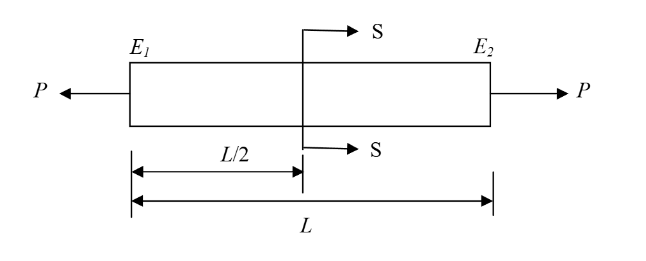
\includegraphics[width=0.5\columnwidth]{figs/1.png}
\caption{}
\label{fig:placeholder}
\end{figure}

\begin{enumerate}
\begin{multicols}{4}
\item $\frac{P}{A}$
\item $\frac{P(E_1-E_2)}{ A(E_1+ E_2)}$
\item $\frac{P E_2}{A E_1}$
\item $\frac{P E_1}{A E_2}$
\end{multicols}
\end{enumerate}

\hfill (GATE PI 2013)

\item For steady, fully developed flow inside a straight pipe of diameter D, neglecting gravity effects, the pressure drop $\Delta p$ over length L and the wall shear stress $tau_w$ are related by 

\begin{enumerate}
\begin{multicols}{4}
\item $\tau_w=\frac{\Delta p D}{4L}$
\item $\tau_w =\frac{\Delta pD^2}{4L^2}$
\item $\tau_w=\frac{ \Delta pD}{2L} $       
\item $\tau_w =\frac{4\Delta pL}{D}  $
\end{multicols}
\end{enumerate}

\hfill (GATE PI 2013)

\item For a ductile material, toughness is a measure of
\begin{enumerate}
\begin{multicols}{2}
\item resistance to scratching 
\item ability to absorb energy up to fracture 
\item ability to absorb energy till elastic limit 
\item resistance to indentation 
\end{multicols}
\end{enumerate}

\hfill (GATE PI 2013)

\item A cube shaped casting solidifies in 5 min. The solidification time in min for a cube of the same material, which is 8 times heavier than the original casting, will be 

\begin{enumerate}
\begin{multicols}{4}
\item 10 
\item 20 
\item 24
\item 40  
\end{multicols}
\end{enumerate}

\hfill (GATE PI 2013)

\item A steel bar 200 mm in diameter is turned at a feed of 0.25 mm/rev with a depth of cut of 4 mm. The rotational speed of the workpiece is 160 rpm. The material removal rate in mm$^3$/s is 

\begin{enumerate}
\begin{multicols}{4}
\item 160
\item 167.6
\item 1600
\item 1675.5  
\end{multicols}
\end{enumerate}

\hfill (GATE PI 2013)

\item In the 3-2-1 principle of fixture design, 3 refers to the number of
\begin{enumerate}
\item clamps required
\item locators on the primary datum face
\item degrees of freedom of the workpiece
\item operations carried out on the primary datum face 
\end{enumerate}

\hfill (GATE PI 2013)

\item In simple exponential smoothing forecasting, to give higher weightage to recent demand information, the smoothing constant must be close to

\begin{enumerate}
\begin{multicols}{4}
\item \--1
\item zero
\item 0.5
\item 1  
\end{multicols}
\end{enumerate}

\hfill (GATE PI 2013)

\item A company manufactures 1000 toys every day. On an average, 10\% of the toys are defective and 40\% of the defective toys can be reworked into defect-free ones. The average number of defect-free toys manufactured daily is 

\begin{enumerate}
\begin{multicols}{4}
\item 900
\item 920
\item 940
\item 960  
\end{multicols}
\end{enumerate}

\hfill (GATE PI 2013)

\item The type of control chart used to monitor the amount of dispersion in a sample is

\begin{enumerate}
\begin{multicols}{4}
\item c-chart
\item p-chart
\item $\Bar{x}$-chart
\item R-chart
\end{multicols}
\end{enumerate}

\hfill (GATE PI 2013)

\item Which one of the following is modeled based on adaptation capabilities of biological systems? 

\begin{enumerate}
\begin{multicols}{2}
\item Relational database 
\item Fuzzy system 
\item Simulated annealing algorithm 
\item Genetic algorithm 
\end{multicols}
\end{enumerate}

\hfill (GATE PI 2013)

\item A company plans to purchase a machine whose uptime needs to be at least 95\%. They have shortlisted two models of the machine with the following operational characteristics: 

\medskip
\begin{table}[htbp]
  \centering
  \caption{Table-3}
  \label{table3}
  \begin{tabular}{cc}
  \textbf{Processing Technique} & \textbf{Producct} \\ \\
    P. Calendering & 1. Pipes \\
    Q. Extrusion & 2. Disposable cups \\
    R. Injection moulding & 3. Sheets \\
    S. Thermoforming & 4. Nylon gears \\
  \end{tabular}
\end{table}

The company should buy
\begin{enumerate}
\begin{multicols}{2}
\item only Model M \item  only Model N 
\item either Model M or N \item  neither Model M nor N 
\end{multicols}
\end{enumerate}

\hfill (GATE PI 2013)

\item A manufacturer produces bars designed to be of 10 mm diameter with a tolerance of $\pm$0.1 mm. Historical data indicates that manufactured bars have an average diameter of 9.98 mm with a standard deviation of 0.15 mm. The process capability index is
\begin{enumerate}
\begin{multicols}{4}
\item 0.08 
\item  0.12 
\item  0.18 
\item 0.27 
\end{multicols}
\end{enumerate}

\hfill (GATE PI 2013)

\item Let (P) denote the linear programming formulation of a transportation problem with $m$ sources and $n$ destinations. Then, the dual linear program of (P) has
\begin{enumerate}
\begin{multicols}{2}
\item $nm$ variables and $nm$ constraints \item  $nm$ variables and $n+m$ constraints 
\item $n+m$ variables and $n+m$ constraints \item $n+m$ variables and $nm$ constraints 
\end{multicols}
\end{enumerate}

\hfill (GATE PI 2013)

\item Following data refers to an automat and a center lathe, which are being compared to machine a batch of parts in a manufacturing shop.

\begin{center}
\begin{tabular}{|c|c|c|}
    \hline
    Task & Task time (Seconds) & Immediate predecessor(s) \\
    \hline
    P & 20 & - \\ \hline
    Q & 25 & P \\  \hline
    R & 10 & Q \\ \hline
    S & 15 & Q \\ \hline 
    T & 25 & R, S \\    \hline
\end{tabular}
\end{center} 

Automat will be economical if the batch size exceeds

\begin{enumerate}
\begin{multicols}{4}
\item 28 
\item 32 
\item 61
\item 75  
\end{multicols}
\end{enumerate}

\hfill (GATE PI 2013)

\item Cylindrical pins of $25.010^{+0.020}_{+0.010}$ mm diameter are electroplated in a shop. Thickness of the plating is $30 \pm 0.2$ microns. Neglecting gage tolerances, the size of the GO gage in mm to inspect the plated components is 

\begin{enumerate}
\begin{multicols}{4}
\item 25.042 
\item 25.052
\item 25.074
\item 25.084
\end{multicols}
\end{enumerate}

\hfill (GATE PI 2013)

\item During the electrochemical machining (ECM) of iron (atomic weight = 56, valency = 2) at a current of 1000 A with 90\% current efficiency, the material removal rate was observed to be 0.26 gm/s. If titanium (atomic weight = 48, valency = 3) is machined by the ECM process at the current of 2000 A with 90\% current efficiency, the expected material removal rate in gm/s will be


\begin{enumerate}
\begin{multicols}{4}
\item 0.11 
\item 0.23
\item 0.30
\item 0.52
\end{multicols}
\end{enumerate}

\hfill (GATE PI 2013)

\item Specific enthalpy and velocity of steam at inlet and exit of a steam turbine, running under steady state, are as given below: \\

\begin{table}[h!]
\centering
\begin{tabular}{|c|c|c|c|}
\hline
\textbf{Pressure} & \textbf{Temperature} & \multicolumn{2}{c|}{\textbf{Specific enthalpy}} \\ \cline{3-4} 
\textbf{(kPa)} & \textbf{($^\circ$C)} & $h_f$ (kJ/kg) & $h_g$ (kJ/kg) \\ \hline
150.9 & $-20$ & 17.82 & 178.74 \\ \hline
500 & 15.6 & 50.64 & 195.01 \\ \hline
\end{tabular}
\end{table}

\bigskip
The rate of heat loss from the turbine per kg of steam flow rate is 5 kW. Neglecting changes in potential energy of steam, the power developed in kW by the steam turbine per kg of steam flow rate is

\begin{enumerate}
\begin{multicols}{4}
\item 901.2 
\item 911.2
\item 17072.5
\item 17082.5
\end{multicols}
\end{enumerate}

\hfill (GATE PI 2013)

\item A simply supported beam of length $L$ is subjected to a varying distributed load $\sin \brak{3\pi x/L}$ Nm$^{-1}$, where the distance $x$ is measured from the left support. The magnitude of the vertical reaction force in N at the left support is

\begin{enumerate}
\begin{multicols}{4}
\item zero 
\item $L/3\pi$
\item  $L/\pi$
\item  $2L/\pi$ 
\end{multicols}
\end{enumerate}

\hfill (GATE PI 2013)


\item The probability that a student knows the correct answer to a multiple choice question is $ \frac{2}{3} $. If the student does not know the answer, then the student guesses the answer. The probability of the guessed answer being correct is $ \frac{1}{4} $. Given that the student has answered the question correctly, the conditional probability that the student knows the correct answer is
\begin{enumerate}
\begin{multicols}{4}
\item $\frac{2}{3} $
\item $\frac{3}{4} $ 
\item  $ \frac{5}{6} $
\item $\frac{8}{9} $ 
\end{multicols}
\end{enumerate}

\hfill (GATE PI 2013)


\item The solution to the differential equation 
\begin{align*}
\frac{d^2 u}{dx^2} - k^2 u = 0
\end{align*}
where $k$ is a constant, subjected to the boundary conditions $u(0) = 0$ and $u(L) = U$, is
\begin{enumerate}
\begin{multicols}{4}
\item $u = \frac{U x}{L}$
\item $u = U (\frac{1 - e^{kx}}{1- e^{kL}})$
\item $u = U (\frac{1 - e^{-kx}}{1- e^{-kL}})$
\item $u = U (\frac{1 + e^{-kx}}{1 + e^{-kL}})$
\end{multicols}
\end{enumerate}

\hfill (GATE PI 2013)

\item The value of the definite integral 
$
\int_1^e \ln(x) \, dx
$
is
\begin{enumerate}
\begin{multicols}{4}
\item $\frac{4\sqrt{e^3}}{9}+ \frac{2}{9}$
\item $\frac{2\sqrt{e^3}}{9} - \frac{4}{9}$
\item $\frac{2\sqrt{e^3}}{9} + \frac{4}{9}$
\item $\frac{4\sqrt{e^3}}{9} - \frac{2}{9}$
\end{multicols}
\end{enumerate}

\hfill (GATE PI 2013)

\item The following surface integral is to be evaluated over a sphere for the given steady velocity vector field  
$
\mathbf{F} = x\mathbf{i} + y\mathbf{j} + z\mathbf{k}
$
where $S$ is the sphere $x^2 + y^2 + z^2 = 1$ and $\mathbf{n}$ is the outward unit normal vector to the sphere:
\begin{align*}
 \iint_S  \frac{1}{4}(\mathbf{F} \cdot \mathbf{n}). dA
\end{align*}
The value of the surface integral is
\begin{enumerate}
\begin{multicols}{2}
\item $\pi$
\item $2\pi$
\item $\frac{3\pi}{4}$
\item $4\pi$
\end{multicols}
\end{enumerate}

\hfill (GATE PI 2013)


\item The function $f(t)$ satisfies the differential equation  
$
\frac{d^2 f}{dt^2} + f = 0
$
and the auxiliary conditions  
$
f(0) = 0 ,\frac{df}{dt}(0) = 4
$
The Laplace transform of $f(t)$ is:
\begin{enumerate}
\begin{multicols}{4}
\item $\frac{2}{s + 1}$
\item $\frac{4}{s + 1}$
\item $\frac{4}{s^2 + 1}$
\item $\frac{2}{s^4 + 1}$
\end{multicols}
\end{enumerate}
\hfill (GATE PI 2013)

\item A flywheel connected to a punching machine has to supply energy of $400$ Nm while running at a mean angular speed of $20$ rad/s. If the total fluctuation of speed is not to exceed $\pm 2\%$, the mass moment of inertia of the flywheel in kg·m$^2$ is
\begin{enumerate}
\begin{multicols}{4}
\item 25
\item 50
\item 100
\item 125
\end{multicols}
\end{enumerate}

\hfill (GATE PI 2013)

\item A single riveted lap joint of two similar plates has the following data: 

    \begin{figure}[h]
    \centering
    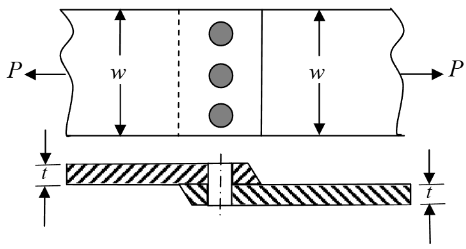
\includegraphics[width=0.5\columnwidth]{figs/2.png}
    \caption{}
    \label{fig:placeholder}
\end{figure} 


Plate width = $200$ mm  \\ Plate thickness = $5$ mm \\ Number of rivets = $3$, Rivet diameter = $10$ mm \\ Rivet hole diameter = $11$ mm \\ Allowable tensile stress of plate $\sigma_p = 200$ MPa \\
Allowable bearing stress of rivet $\sigma_c = 150$ MPa.  

If the plates are designed to avoid tearing failure, the maximum permissible load $P$ in kN is
\begin{enumerate}
\begin{multicols}{2}
\item 83
\item 125
\item 167
\item 501
\end{multicols}
\end{enumerate}

\hfill (GATE PI 2013)

\item Two cutting tools are being compared for a machining operation. The tool life equations are:  
\begin{align*}
\text{Carbide tool}: VT^{1.6} = 3000 \\  
\text{HSS tool}: VT^{0.6} = 200  
\end{align*}
where $V$ is cutting speed in m/min and $T$ is tool life in min. The carbide tool will provide higher tool life if the cutting speed in m/min exceeds
\begin{enumerate}
\begin{multicols}{4}
\item 15.0
\item 39.4
\item 49.3
\item 60.0
\end{multicols}
\end{enumerate}

\hfill (GATE PI 2013)


\item In a CAD package, mirror image of a 2D point $P\brak{5,10}$ is to be obtained about a line which passes through the origin and makes an angle of $45^\circ$ counterclockwise with the X-axis. The coordinates of the transformed point will be
\begin{enumerate}
\begin{multicols}{4}
\item (7.5, 5)
\item (10, 5)
\item (7.5, \--5)
\item (10, \--5)
\end{multicols}
\end{enumerate}

\hfill (GATE PI 2013)

\item In water jet machining, the water jet is issued through a $0.3$ mm diameter orifice at a pressure of $400$ MPa. The density of water is $1000 \ \text{kg/m}^3$. The coefficient of discharge is $1.0$. Neglecting all losses during water jet formation through the orifice, the power of the water jet in kW is
\begin{enumerate}
\begin{multicols}{4}
\item 25.3
\item 50.6
\item 75.9
\item 101.2
\end{multicols}
\end{enumerate}

\hfill (GATE PI 2013)

\item A linear programming problem is shown below: 

Maximize 
\begin{align*}
3x + 7y
\end{align*}
Subject to:  
\begin{align*}
3x + 7y \leq 10 \\
4x + 6y \leq 8  \\
x, y \geq 0 \\
\end{align*}
It has:
\begin{enumerate}
\begin{multicols}{2}
\item an unbounded objective function
\item exactly one optimal solution
\item exactly two optimal solutions
\item infinitely many optimal solutions
\end{multicols}
\end{enumerate}

\hfill (GATE PI 2013)

\item Consider a two\--machine flow shop where jobs are first processed in Machine X and then in Machine Y, in the same sequence.  
The processing times of four jobs (1, 2, 3 and 4) on the machines are:   
\begin{table}[htbp]
  \centering
  \caption{Table-6}
  \label{tab:tables/table6.tex}
  \begin{tabular}{cc}
  \textbf{Reagent} & \textbf{Function} \\ \\
    P.Ammonia  & 1. Prevent storage hardening \\
    Q. Hydroxylamine & 2. Delay plugging mechanism \\
    R. Formic acid & 3. Stabilizer \\
    S. Ethephone & 4. Coagulating agent \\
  \end{tabular}
\end{table}
The sequence of jobs on the machines that minimizes make span is:
\begin{enumerate}
\begin{multicols}{4}
\item 2--3--1--4
\item 1--2--3--4
\item 2--1--3--4
\item 3--1--4--2
\end{multicols}
\end{enumerate}

\hfill (GATE PI 2013)


\item Match the CORRECT pairs:  
\begin{table}[htbp]
  \centering
  \caption{Table-7}
  \label{tab:tables/table7.tex}
  \begin{tabular}{cc}
\textbf{Additives} & \textbf{Fuction}\\

P. Molybdenum disulphide & 1. Heat stabilizer \\
Q. Glycerol monostearate & 2. UV-absorber \\
R. Tribasic lead sulphate & 3. Antistatic agent \\
S. 2-hydroxybenzophenone & 4. Solid layer lubricant \\
  
  
  
  \end{tabular}
\end{table} 

\begin{enumerate}
\begin{multicols}{2}
\item P-2, Q-3, R-4, S-1
\item P-3, Q-2, R-4, S-1
\item P-4, Q-1, R-3, S-2
\item P-4, Q-3, R-1, S-2
\end{multicols}
\end{enumerate}

\hfill (GATE PI 2013)

\item A firm produces $120$ units of product in every $8$\--hour shift. Four operations as given below are needed to manufacture each unit: 

\begin{table}[htbp]
  \centering
  \caption{Table-8}
  \label{table8}
  \begin{tabular}{cc}
  \textbf{Group-I} & \textbf{Group-II} \\ \\
    P. Corn & 1. Lycopene \\
    Q. Red pepper & 2. $\beta$-Carotene \\
    R. Pumpkin & 3. Capsanthin \\
    S. Tomato & 4. Lutein \\
  \end{tabular}
\end{table} 

The above operations are to be assigned to workstations such that one or more operations are performed in each workstation.  
Only one unit of product will be processed in each workstation at a time.  
The minimum number of workstations that will achieve the production target, without violating the precedence constraints, is:
\begin{enumerate}
\begin{multicols}{4}
\item 1
\item 2
\item 3
\item 4
\end{multicols}
\end{enumerate}

\hfill (GATE PI 2013)

\textbf{\large{Common Data Questions}} \\
\textbf{Common Data for Questions 48 and 49:}\\
 
 A disc of $200$ mm outer and $80$ mm inner diameter is faced at a feed of $0.1$ mm/rev with a depth of cut of $1$ mm. The facing operation is undertaken at a constant cutting speed of $90$ m/min in a CNC lathe. The main (tangential) cutting force is $200$ N.  \\

\item Neglecting the contribution of the feed force towards cutting power, the specific cutting energy in J/mm$^3$ is:
\begin{enumerate}
\begin{multicols}{4}
\item 0.2
\item 2
\item 200
\item 2000
\end{multicols}
\end{enumerate}


\hfill (GATE PI 2013)

\item Assuming approach and over\--travel of the cutting tool to be zero, the machining time in minutes is:
\begin{enumerate}
\begin{multicols}{4}
\item 2.93
\item 5.86
\item 6.66
\item 13.33
\end{multicols}
\end{enumerate}

\hfill (GATE PI 2013)

\textbf{Common Data for Questions 50 and 51:} \\

The demand for soap at a retailer is 40 kg per day. The retailer buys soap in bulk at a cost of Rs. 50 per kg.  
The ordering cost is Rs. 200 per order and the holding cost is Rs. 0.1 per kg per day. The lead time is 3 days.  
The retailer's current policy is to order 200 kg every 5 days.  \\  
\item To avoid stock\--out situations, the retailer needs to place orders when the inventory level (in kg) drops to:
\begin{enumerate}
\begin{multicols}{4}
\item 40
\item 60
\item 80
\item 120
\end{multicols}
\end{enumerate}

\hfill (GATE PI 2013)

\item If the retailer uses an optimum policy to minimize the total cost,the saving in Rs. in the total cost as compared to the current policy will be
\begin{enumerate}
    \begin{multicols}{4}
    \item 10
    \item 20 
    \item 40 
    \item 50 
    \end{multicols}
\end{enumerate}

\hfill (GATE PI 2013)

\textbf{Linked Answer Questions}

\textbf{Statement for Linked Answer Questions 52 and 53:}  

A project consists of seven activities, whose durations are independent normal random variables, as shown in the table below. Activities are identified by their beginning node $i$ and ending node $j$. \\

\begin{table}[htbp]
  \centering
  \caption{Table-9}
  \label{tab:tables/table9.tex}
  \begin{tabular}{cc}
  \textbf{Group-I} & \textbf{Group-II} \\ \\
    P. Degumming & 1. Crystallization of triacylglycerol by cooling to remove fat crystals \\
    Q. Deacidifying & 2. Passing heated oil over charcoal \\
    R. Bleaching & 3. Using alkaline solution to remove fatty acids \\
    S. Winterizing & 4. Wetting with water to remove lecithin \\
  \end{tabular}
\end{table}
\newline
\item The critical path of the project, based on the mean activity duration, is:
\begin{enumerate}
\begin{multicols}{4}
\item $1 - 2 - 3 - 4 - 5$
\item $1 - 2 - 3 - 5$
\item $1 - 3 - 5$
\item $1 - 3 - 4 - 5$
\end{multicols}
\end{enumerate}

\hfill (GATE PI 2013)

\item Let $\Phi$ denote the cumulative distribution function of the standard normal random variable. The probability that all activities on the critical path, based on the mean activity duration, are completed in 22 days is:
\begin{enumerate}
\begin{multicols}{4}
\item $\Phi^{-1}\brak{0.333}$
\item $\Phi^{-1}\brak{0.816}$
\item $\Phi^{-1}\brak{1.664}$
\item $\Phi^{-1}\brak{2.235}$
\end{multicols}
\end{enumerate}

\hfill (GATE PI 2013)

\textbf{Statement for Linked Answer Questions 54 and 55:}  

In orthogonal turning of a bar of 100 mm diameter with a feed of 0.25 mm/rev, depth of cut of 4 mm, and cutting velocity of 90 m/min, it is observed that the main (tangential) cutting force is perpendicular to the friction force acting at the chip-tool interface. The main (tangential) cutting force is 1500 N. \\

\item The orthogonal rake angle of the cutting tool in degrees is:
\begin{enumerate}
\begin{multicols}{4}
\item zero
\item 3.58
\item 5
\item 7.16
\end{multicols}
\end{enumerate}

\hfill (GATE PI 2013)

\item The normal force acting at the chip-tool interface in N is:
\begin{enumerate}
\begin{multicols}{4}
\item 1000
\item 1500
\item 2000
\item 2500
\end{multicols}
\end{enumerate}

\hfill (GATE PI 2013)

\textbf{General Aptitude (GA) Questions} \\

\item Were you a bird, you ............. in the sky.
\begin{enumerate}
\item would fly
\item shall fly
\item should fly
\item shall have flown
\end{enumerate}


\hfill (GATE PI 2013)

\item Choose the grammatically INCORRECT sentence:
\begin{enumerate}
\begin{multicols}{2}
\item He is of Asian origin.
\item They belonged to Africa.
\item She is an European.
\item They migrated from India to Australia.
\end{multicols}
\end{enumerate}

\hfill (GATE PI 2013)

\item Complete the sentence:  
Universalism is to particularism as diffuseness is to ................
\begin{enumerate}
\begin{multicols}{4}
\item specificity
\item neutrality
\item generality
\item adaptation
\end{multicols}
\end{enumerate}

\hfill (GATE PI 2013)


\item What will be the maximum sum of $44, 42, 40, \ldots$ ?
\begin{enumerate}
\begin{multicols}{4}
\item 502
\item 504
\item 506
\item 500
\end{multicols}
\end{enumerate}

\hfill (GATE PI 2013)

\item Which one of the following options is the closest in meaning to the  word given below? \\ 
\textbf{Nadir}
\begin{enumerate}
\begin{multicols}{4}
\item Highest
\item Lowest
\item Medium
\item Integration
\end{multicols}
\end{enumerate}

\hfill (GATE PI 2013)

\textbf{Q.61 to Q.65 carry two marks each} \\

\item A tourist covers half of his journey by train at $60$ km/h, half of the remainder by bus at $30$ km/h and the rest by cycle at $10$ km/h.  
The average speed of the tourist in km/h during his entire journey is:
\begin{enumerate}
\begin{multicols}{4}
\item 36
\item 30
\item 24
\item 18
\end{multicols}
\end{enumerate}

\hfill (GATE PI 2013)


\item The current erection cost of a structure is Rs. $13{,}200$.  
If the labour wages per day increase by 1/5 of the current wages and the working hours decrease by 1/24 of the current period, then the new cost of erection in Rs. is:
\begin{enumerate}
\begin{multicols}{4}
\item 16,500
\item 15,180
\item 11,000
\item 10,120
\end{multicols}
\end{enumerate}


\hfill (GATE PI 2013)

\item Out of all the 2-digit integers between 1 and 100, a 2-digit number has to be selected at random.  
What is the probability that the selected number is not divisible by $7$?
\begin{enumerate}
\begin{multicols}{4}
\item 13/90
\item 12/90
\item 78/90
\item 77/90
\end{multicols}
\end{enumerate}

\hfill (GATE PI 2013)

\item After several defeats in wars, Robert Bruce went in exile and wanted to commit suicide. Just before committing suicide, he came across a spider attempting tirelessly to have its net. Time and again, the spider failed but that did not deter it from making attempts. Such attempts by the spider made Bruce curious. Thus, Bruce started observing the near-impossible goal of the spider to have the net. Ultimately, the spider succeeded in having its net despite several failures. Such act of the spider encouraged Bruce not to commit suicide. And then, Bruce went back again and won many a battle, and the rest is history.  \\\  

Which one of the following assertions is best supported by the above information? \\
\begin{enumerate}
\item Failure is the pillar of success.
\item Honesty is the best policy.
\item Life begins and ends with adventures.
\item No adversity justifies giving up hope. 
\end{enumerate}

\hfill (GATE PI 2013)

\item Find the sum of the expression  

81 + 80 + 1 + ...... + 4 + 3 + 1 + 3 + 2 + 1 + 2 + 1 + 1
\begin{enumerate}
\begin{multicols}{2}
\item 7
\item 8
\item 9
\item 10
\end{multicols}
\end{enumerate}

\hfill (GATE PI 2013)
\end{enumerate}


\end{document}